\documentclass[7pt]{article}
\usepackage[utf8]{inputenc}

% This is a helpful package that puts math inside length specifications
\usepackage{multirow}
\usepackage{url}
\usepackage{calc}
\usepackage[spanish, es-tabla]{babel}
\usepackage{graphicx}
\usepackage{xcoffins}
\usepackage{array}
\usepackage{multicol}
\usepackage{multirow}
%\usepackage[latin1]{inputenc}


% Layout: Puts the section titles on left side of page
\reversemarginpar

%
%         PAPER SIZE, PAGE NUMBER, AND DOCUMENT LAYOUT NOTES:
%
% The next \usepackage line changes the layout for CV style section
% headings as marginal notes. It also sets up the paper size as either
% letter or A4. By default, letter was used. If A4 paper is desired,
% comment out the letterpaper lines and uncomment the a4paper lines.
%
% As you can see, the margin widths and section title widths can be
% easily adjusted.
%
% ALSO: Notice that the includefoot option can be commented OUT in order
% to put the PAGE NUMBER *IN* the bottom margin. This will make the
% effective text area larger.
%
% IF YOU WISH TO REMOVE THE ``of LASTPAGE'' next to each page number,
% see the note about the +LP and -LP lines below. Comment out the +LP
% and uncomment the -LP.
%
% IF YOU WISH TO REMOVE PAGE NUMBERS, be sure that the includefoot line
% is uncommented and ALSO uncomment the \pagestyle{empty} a few lines
% below.
%

%% Use these lines for letter-sized paper
\usepackage[paper=letterpaper,
            %includefoot, % Uncomment to put page number above margin
            marginparwidth=1.0in,     % Length of section titles
            marginparsep=.05in,       % Space between titles and text
            margin=1in,               % 1 inch margins
            includemp]{geometry}

%% Use these lines for A4-sized paper
%\usepackage[paper=a4paper,
%            %includefoot, % Uncomment to put page number above margin
%            marginparwidth=30.5mm,    % Length of section titles
%            marginparsep=1.5mm,       % Space between titles and text
%            margin=25mm,              % 25mm margins
%            includemp]{geometry}

%% More layout: Get rid of indenting throughout entire document
\setlength{\parindent}{0in}

%% This gives us fun enumeration environments. compactitem will be nice.
\usepackage{paralist}

%% Reference the last page in the page number
%
% NOTE: comment the +LP line and uncomment the -LP line to have page
%       numbers without the ``of ##'' last page reference)
%
% NOTE: uncomment the \pagestyle{empty} line to get rid of all page
%       numbers (make sure includefoot is commented out above)
%
\usepackage{fancyhdr,lastpage}
\pagestyle{fancy}
%\pagestyle{empty}      % Uncomment this to get rid of page numbers
\fancyhf{}\renewcommand{\headrulewidth}{0pt}
\fancyfootoffset{\marginparsep+\marginparwidth}
\newlength{\footpageshift}
\setlength{\footpageshift}
          {0.5\textwidth+0.5\marginparsep+0.5\marginparwidth-2in}
\lfoot{\hspace{\footpageshift}%
       \parbox{4in}{\, \hfill %
                    \arabic{page} / \protect\pageref*{LastPage} % +LP
%                    \arabic{page}                               % -LP
                    \hfill \,}}

% Finally, give us PDF bookmarks
\usepackage{color,hyperref}
\definecolor{darkblue}{rgb}{0.0,0.0,0.3}
\hypersetup{colorlinks,breaklinks,
            linkcolor=darkblue,urlcolor=darkblue,
            anchorcolor=darkblue,citecolor=darkblue}

%%%%%%%%%%%%%%%%%%%%%%%% End Document Setup %%%%%%%%%%%%%%%%%%%%%%%%%%%%


%%%%%%%%%%%%%%%%%%%%%%%%%%% Helper Commands %%%%%%%%%%%%%%%%%%%%%%%%%%%%

% The title (name) with a horizontal rule under it
%
% Usage: \makeheading{name}
%
% Place at top of document. It should be the first thing.
\newcommand{\makeheading}[1]%
        {\hspace*{-\marginparsep minus \marginparwidth}%
         \begin{minipage}[t]{\textwidth+\marginparwidth+\marginparsep}%
                {\large \bfseries #1}\\[-0.15\baselineskip]%
                 \rule{\columnwidth}{1pt}%
         \end{minipage}}

% The section headings
%
% Usage: \section{section name}
%
% Follow this section IMMEDIATELY with the first line of the section
% text. Do not put whitespace in between. That is, do this:
%
%       \section{My Information}
%       Here is my information.
%
% and NOT this:
%
%       \section{My Information}
%
%       Here is my information.
%
% Otherwise the top of the section header will not line up with the top
% of the section. Of course, using a single comment character (%) on
% empty lines allows for the function of the first example with the
% readability of the second example.
\renewcommand{\section}[2]%
        {\pagebreak[2]\vspace{1.3\baselineskip}%
         \phantomsection\addcontentsline{toc}{section}{#1}%
         \hspace{0in}%
         \marginpar{
         \raggedright \scshape #1}#2}

% An itemize-style list with lots of space between items
\newenvironment{outerlist}[1][\enskip\textbullet]%
        {\begin{itemize}[#1]}{\end{itemize}%
         \vspace{-.6\baselineskip}}

% An environment IDENTICAL to outerlist that has better pre-list spacing
% when used as the first thing in a \section 
\newenvironment{lonelist}[1][\enskip\textbullet]%
        {\vspace{-\baselineskip}\begin{list}{#1}{%
        \setlength{\partopsep}{0pt}%
        \setlength{\topsep}{0pt}}}
        {\end{list}\vspace{-.6\baselineskip}}

% An itemize-style list with little space between items
\newenvironment{innerlist}[1][\enskip\textbullet]%
        {\begin{compactitem}[#1]}{\end{compactitem}}

% To add some paragraph space between lines.
% This also tells LaTeX to preferably break a page on one of these gaps
% if there is a needed pagebreak nearby.
\newcommand{\blankline}{\quad\pagebreak[2]}

%%%%%%%%%%%%%%%%%%%%%%%% End Helper Commands %%%%%%%%%%%%%%%%%%%%%%%%%%%

%%%%%%%%%%%%%%%%%%%%%%%%% Begin CV Document %%%%%%%%%%%%%%%%%%%%%%%%%%%%

\newcolumntype{M}[1]{>{\centering\arraybackslash}m{#1}}
\newcolumntype{P}[1]{>{\hfill\arraybackslash}p{#1}}

\begin{document}
\small{
\makeheading{Dr. Rodrigo L\'{o}pez Far\'{i}as (Updated: \textit{29 / Feb / 2016} )}  

\section{Personal Information} %\newlength{\rcollength}\setlength{\rcollength}{2.3in}%
%
%+393204884472
\begin{tabular}{l P{70mm} M{20mm}}
{Birthday: 8 / Jul / 1984} 		& 		 	Cellular: +52 4431555416					& \multirow{4}{*}[1.3cm]{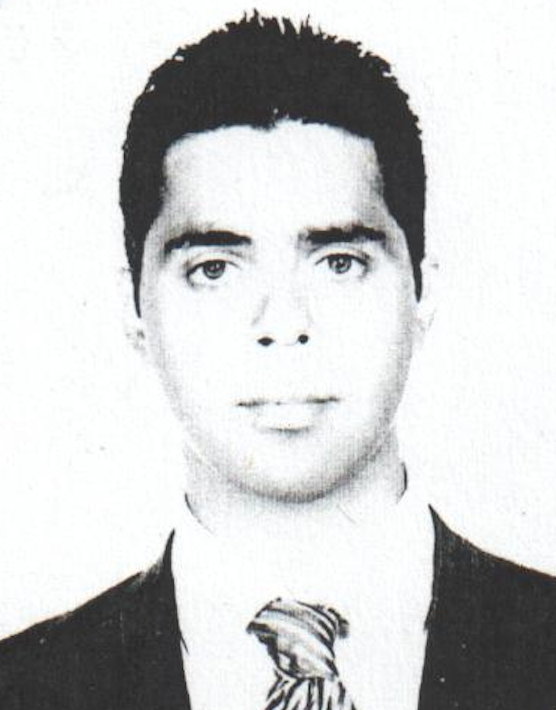
\includegraphics[width=2.4cm]{foto.png}  } 	\\
{Address: Aram\'{e}n \# 313}	&     	  	e-mail: rodrigo.lopez@alumni.imtlucca.it 	&	\\
CP: 58070           			& 			Skype ID: rdglpz					&	\\
Morelia, Mexico         		&		 												&
\end{tabular}


\section{Interests \& Skills  } \textbf{Programming Lenguages} 

Matlab, MATHEMATICA, R, Java, C/C++, PHP, HTML, MySQL, Python, LISP.


%\blankline


\textbf{Research} 


 Machine learning Data mining, Dimensionality reduction, Machine Learning, Time series, Nonlinear dynamical systems, Global optimization, Evolutionary computing.
 
 
\textbf{Languages} 

English: 550 TOEFL points. Italian: B1 Common CEFRL Level 




\section{Academic Degree} {\textbf{PhD in Computer Science and Engineering }}(W. European Doctorate mention). Lucca, Italy. (February 2012 - January 2016)


\textbf{Institute of Advanced Studies Lucca}
		\begin{outerlist}
			\item Thesis: Time Series Forecasting Based on Classification of Dynamic Patterns.
			 \begin{innerlist}
                 \item  {Advisors: Dr. Alberto Bemporad. Dr. Pantelis Sopasakis}
        	\item Study field: Time series analysis.
	    \end{innerlist}
		\end{outerlist}
		
\blankline

		{\textbf{MSc in Electrical Engineering (Branch: Computational Systems)}}. \textit{Morelia, Mexico. ( March 2008 - August 2010)}
		
		
	\textbf{Univesidad Michoacana de San Nicolas de Hidalgo}
	

	\begin{outerlist}
	
        	\item Thesis: Bifurcation Diagrams for Discontinuous or Non-differentiable Equations.
	    \begin{innerlist}
                 \item  {Advisors: Dr. Juan Jose Flores Romero, Dr. Claudio Fuerte E.}
        	\item Keywords: Evolutionary computing, nonlinear dynamical systems, stability analysis and optimization.
	    \end{innerlist}
\end{outerlist}

%

\blankline


{\textbf{Engineer in Computational Systems}}. 
\textit{Morelia, Mexico (2002-2007)}

\textbf{Instituto Tecnologico de Morelia}

\begin{outerlist}
	
        	\item Thesis: Implementation and performance analysis of \textbf{``Linux Terminal Server Project"} for educational purposes.
	    \begin{innerlist}
        	\item Topic: Distributed operative Systems.
	    \end{innerlist}
\end{outerlist}


\section{Academic Experience}  {\textbf{Instituto Tecnol\'{o}gico de Morelia}}.
Morelia, Mexico.

\begin{outerlist}

\item[] 


\textit{Teaching}%
\hfill \textbf{August 2011 - January 2012}
\begin{innerlist}
\item Structured and Object Oriented Computer programming (In Electronic and  Industrial Engineering), Research Methodology (In Computational Systems Engineering).  
\end{innerlist}

\hfill \textbf{January 2011 - July 2011}
	\begin{innerlist}
		%\item Professor of: Database Fundamentals (Computational Systems Engineering), Structures and organization of Data (�Technology Information Engineering) and Evaluation of Software Projects (Informatics).  
		\item Database Fundamentals (Computational Systems Engineering), Structures and organization of data. (Technology Information Engineering) and Evaluation of software projects.
		\end{innerlist}
		
		\hfill \textbf{August 2010 - December 2010}
	\begin{innerlist}
		\item  Operative systems, selected topics of programming and research fundamentals.
	\end{innerlist}
%	\hfill \textbf{August 2011 - December 2011}
	%\begin{innerlist}
		%\item Operative Systems II, Programming and Algorithms, Programming II (Object Oriented Programming).	
	%\hfill \textbf{January 2011 - July 2011}
	%\begin{innerlist}
	%	\item Database fundamentals, Programming, Evaluation of software projects.
	%\end{innerlist}	
	%\hfill \textbf{August 2010 - December 2010}
	%\begin{innerlist}
	%	\item Operative systems, selected topics programming, research fundamentals.
	%\end{innerlist}
\end{outerlist}



{\textbf{Universidad de Morelia}}.
Morelia, Mexico.
\begin{outerlist}

\item[] 
\textit{Teaching}%
\hfill \textbf{August 2009 - December 2009}

\begin{innerlist}
	\item Web programming with PHP
\end{innerlist}

\end{outerlist}




\blankline

\section{Professional Experience}
%\subsection{Participation in Research Projects}
\textbf{State Center for Information and Communications Technologies (CETIC)}.
Morelia, Mexico.

\begin{outerlist}
\item[] \textit{Resident in physical infrastructure}%
        \hfill \textbf{March 2007 - June 2007}
\begin{innerlist}
\item Performance analysis of \textbf{Linux Terminal Server Project} applied to to basic education.
%\item Implementación para análisis de rendimiento y alcances de `\textbf{Linux Terminal Server Project}`.

\end{innerlist}
\end{outerlist}
\blankline

{\textbf{Instituto Tecnologico de Morelia}}.
Morelia, Mexico.

\begin{outerlist}
\item[] \textit{Social Service Project}%
        \hfill \textbf{February 2007}
\begin{innerlist}
\item Develop of a PHP Web catalog for Social Service.
%\item Elaboración de un catálogo electrónico web para el Servicio Social.

\end{innerlist}
\end{outerlist}

\begin{outerlist}
\item[] \textit{IMPULSA}%
        \hfill \textbf{May 2005}
\begin{innerlist}
\item Young entrepreneurs program: IMPULSA.
%\item Programa de Jóvenes emprendedores IMPULSA como Director de Finanzas.
\end{innerlist}

\end{outerlist}

\blankline

\section{Publications} \textbf{Journal Articles}
\blankline

%\subsection{Journal Articles Sent}
\begin{innerlist}
\item \textit{Hector Rodriguez Rangel, Vicenc Puig,Rodrigo L\'{o}pez Far\'{i}as, Juan J. Flores }  Short Term Demand Forecast using Bank of Neural Network Models Trained using Genetic Algorithms for the Optimal Management of Drinking Water Networks.  \textit{Engineering Applications of Artificial Intelligence}. \textit{Under review}.
\end{innerlist}


\blankline



\textbf{Peer Reviewed Accepted Conference Articles}




\begin{innerlist}

\item \textit{Rodrigo L\'{o}pez Far\'{i}as, Juan J. Flores and Vicenc Puig}.  Qualitative and Quantitative Multi-Model Forecasting with Nonlinear Noise Filter Applied to Water Demand \textit{IEEE Autumn Meeting on Power, Electronics and Computing} \textbf{Ixtapa M\'{e}xico, November 2015 }.


\item \textit{Juan J. Flores, Jose Ortiz Bejar, Jose Rafael Cedeno, Carlos Lara-Alvarez and Rodrigo L\'{o}pez Far\'{i}as} FNN a Fuzzy Version of the Nearest Neighbour Time Series Forecasting Technique \textit{IEEE Autumn Meeting on Power, Electronics and Computing} \textbf{Ixtapa M\'{e}xico, November 2015 }.


\item \textit{Rodrigo L\'{o}pea Far\'{i}as, Vicenc Puig}   A Multiple-Model Predictor Approach Based on an On-Line Mode Recognition with Application to Water Demand Forecasting \textit{International work-conference on Time Series 1 
} \textbf{Granada Espa\~na, July 2015}.

\item \textit{Rodrigo. L\'{o}pez, V. Puig, H. Rodriguez}   An implementation of a multi-model predictor based on the qualitative and quantitative decomposition of the time-series \textit{International work-conference on Time Series 1 
} \textbf{Granada Espa\~na, July 2015}.

\item \textit{Dr, Juan Flores, Rodrigo López, Julio Barrera.} Optimization with gravitational Interactions  \textit{ROPEC XIII: Autumn Meeting of Electric power systems, electronic and computation (Reuni\'{o}n de Oto\~no de Potencia, Electr\'{o}inca y Computaci\'{o}n)} \textbf{Morelia M\'{e}xico, Noviembre 2011}.

\item Juan Flores, Rodrigo Lopez, Julio Barrera. Gravitational Interactions Optimization. In \textit{Learning and Intelligent OptimizatioN}  (LION 5) \textbf{Roma, Italy - January 2011}.

\item Juan J. Flores, Rodrigo Lopez and Julio Barrera. Particle swarm optimization with gravitational interactions for multimodal and unimodal problems. In \textit{Proceedings of the 9th Mexican International Conference on Artificial Intelligence (MICAI 2010)}, pages 361–370. Springer-Verlag. \textbf{Pachuca, México. November 2010.}

\end{innerlist}




\section{Conferences, Seminars \& Workshops } \textbf{Given} \begin{innerlist}
 %\item Learning and Intelligent OptimizatioN - 'Gravitational Interactions Optimization'. (Rome, Italy. January 2011)
 \item 10mo Congreso Estatal de Ciencia, Tecnolog\'{i}a e Innovaci\'{o}n, en  Ciencias de la Ingenier\'{i}a y Tecnolog\'{i}a. PSO con Nichos Interactivos y B\'{u}squedas locales con Quasi-Newton  (Morelia, México. September 2015 )
 \item Activities of X Anniversary of the Instituto Tecnológico Superior de Ciudad Hidalgo -'Evolutionary computing applied to dynamical systems'.(Morelia, México. October 2010).
\item Week of Research Projects FIE of the UMSNH - 'Gravitational Interactions Optimization'(Morelia, México. June 2010 ).
\item Week of Research Projects FIE of the UMSNH - 'Bifurcations Diagrams using Artificial Intelligence Tools'(Morelia, México. June 2009).
\end{innerlist}



}

\blankline

\textbf{Attended}
\begin{innerlist}
\item 5th HYCON2 Ph.D. School on Control of Networked and Large-Scale Systems and the EFFINET Ph.D. School on Control of Drinking Water Networks  (Lucca Italy, 1-5 of July 2013)
\item Java workshop in the 2nd Week of Computation and Systems. \textit{Morelia, Mexico (2006).}
\item Analysis and Object Oriented Design using UML  (Morelia Mexico,  8-12 of August 2011)

%\item Taller de Java en la 2da Semana de Sistemas y Computación (Morelia México, 2006)
%\item Week of Systems and computation in the Instituto Tecnológico de Morelia. \textit{Morelia, México (2006)}.
%\item 2da. Semana de Sistemas y Computaci\'on en el Instituto Tecnológico de Morelia (Morelia México, 2006).	
%\item Week of Systems and computation in the Instituto Tecnológico de Morelia. \textit{Morelia, México (2005).}
\end{innerlist}
\end{document}




%%%%%%%%%%%%%%%%%%%%%%%%%% End CV Document %%%%%%%%%%%%%%%%%%%%%%%%%%%%%
